\subsection{Esatriene}

La molecola di esatriene \`e stata presa in esame sugli stessi parametri
dell'etilene, considerando la rotazione attorno al doppio legame centrale.

\begin{figure}[ht]
\begin{center}
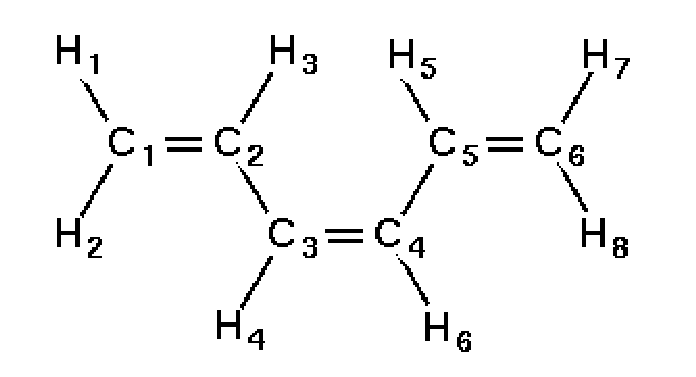
\includegraphics[angle=0,width=6cm,keepaspectratio]{immagini/esatriene/esatriene_cis.eps}
\end{center}
\end{figure}

Si \`e infatti valutata la superficie di potenziale associata ai due gradi di libert\`a
definiti dagli angoli diedri \mbox{C$_2$-C$_3$-C$_4$-C$_5$} e \mbox{H$_4$-C$_3$-C$_4$-H$_6$}.
La base usata per questa trattazione \`e la {6-31G*}. Lo spazio CAS \`e stato
definito in modo tale da includere 6 orbitali $\pi$ ed i corrispondenti
6 elettroni.
\begin{figure}[ht]
\begin{center}
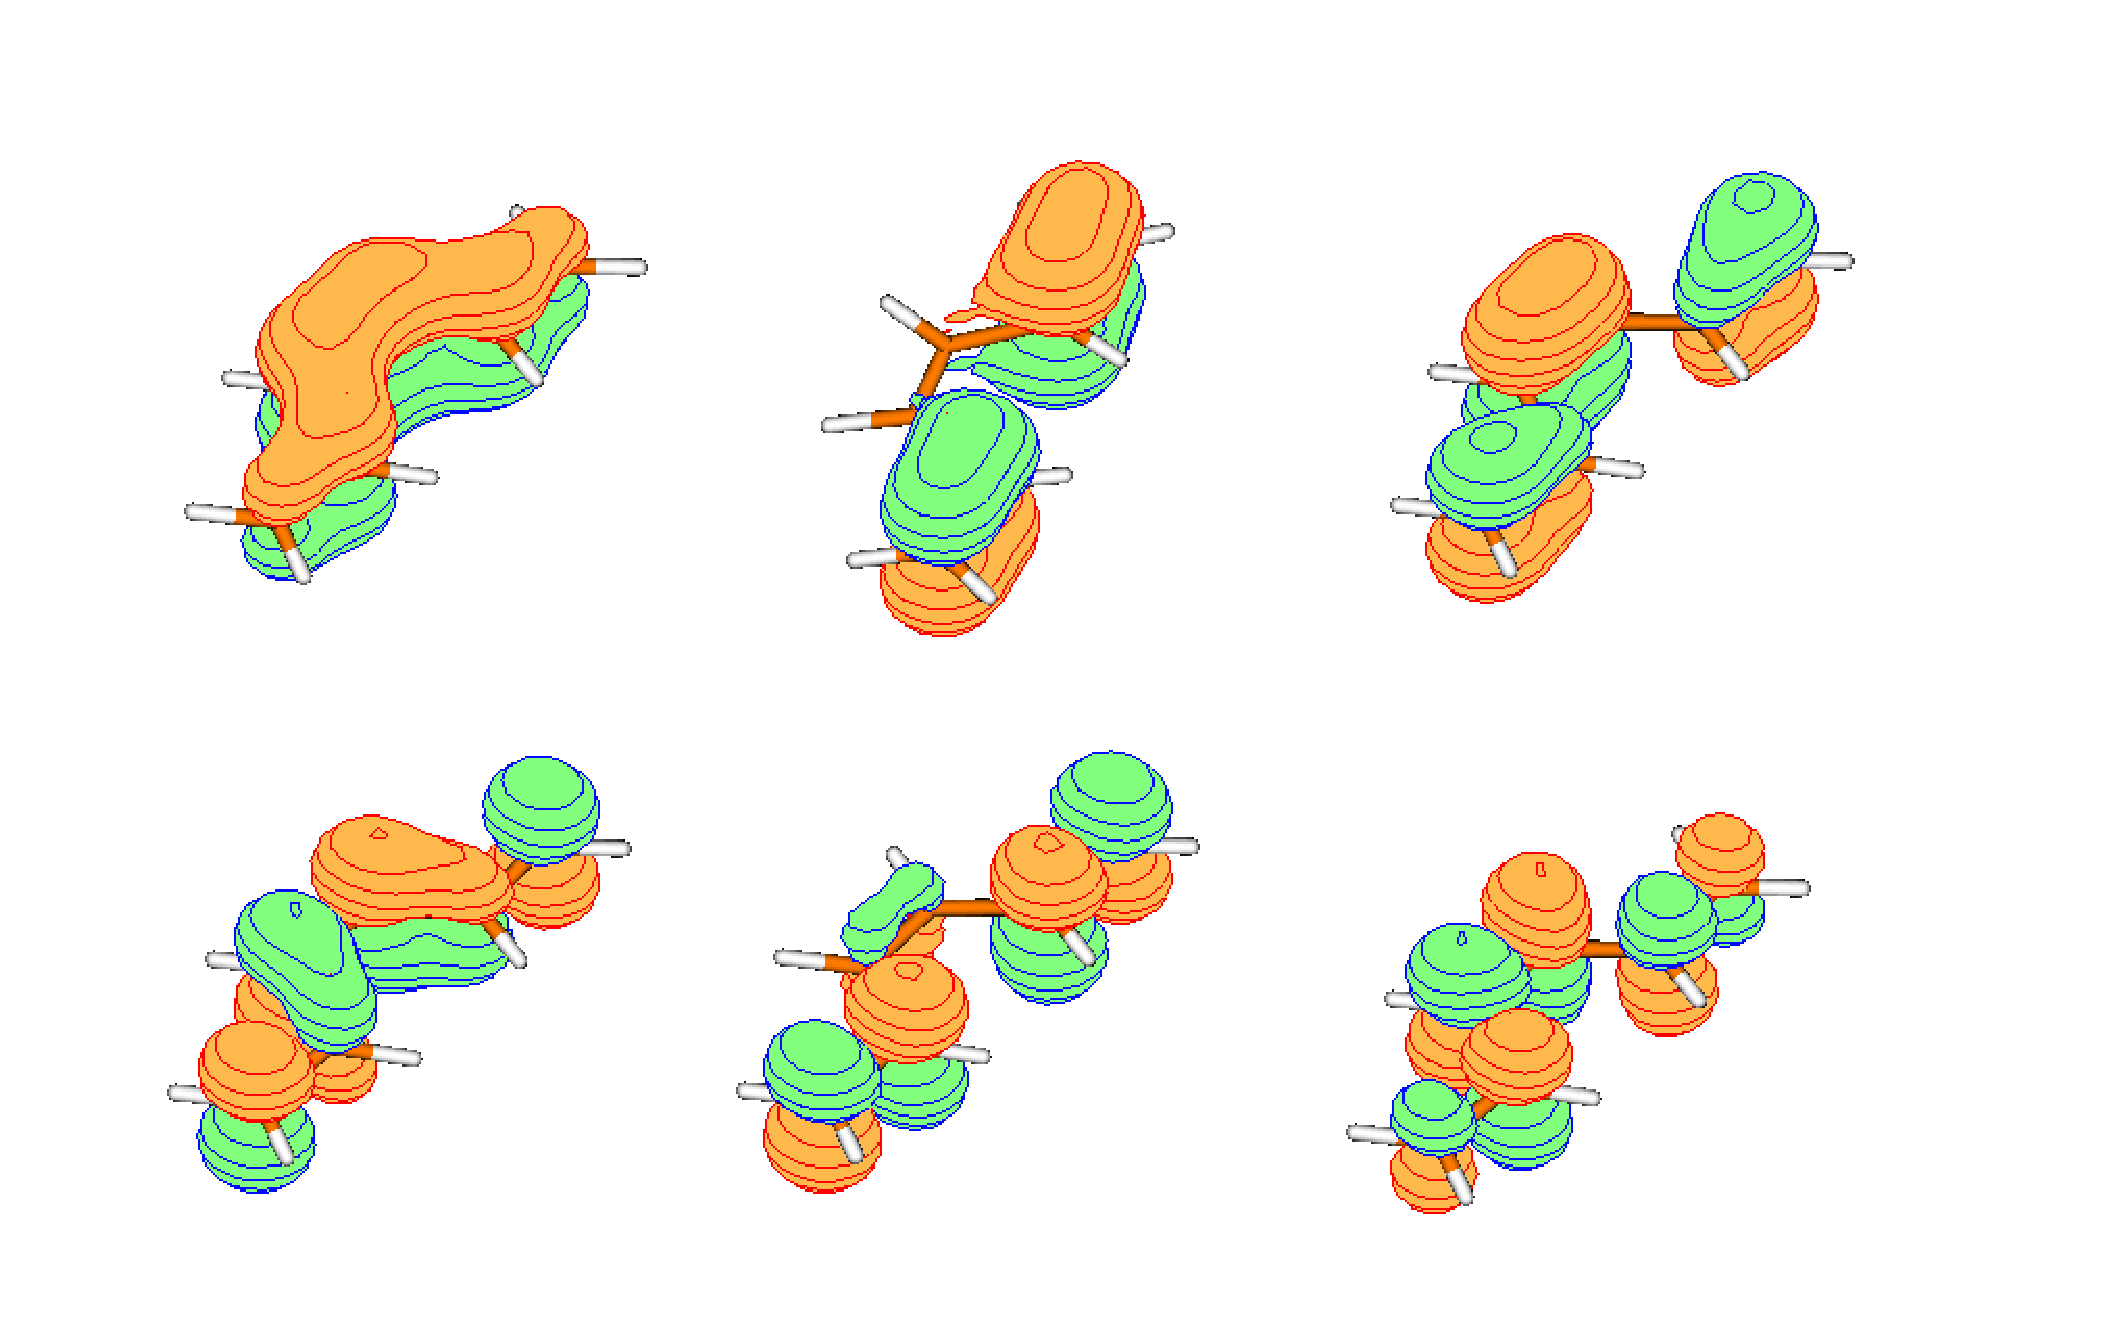
\includegraphics[angle=0,width=10cm,keepaspectratio]{immagini/esatriene/orbitali.eps}
\caption{\small Esatriene cis - orbitali nello spazio CAS 6/6}
\label{fig:esatriene_orbitali}
\end{center}
\end{figure}

\clearpage

La geometria dell'esatriene cis all'equilibrio \`e definita in tabella
\ref{tab:esatriene_geometrie}.
\begin{center}
\begin{threeparttable}
\caption{\small Esatriene cis - geometria stato fondamentale}
\label{tab:esatriene_geometrie}
\small
\begin{tabular}{|ccc|c|}
\hline
							& CASSCF	& Exp.\tnote{1} \\ 
\hline
$r$(C$_1$=C$_2$)			& 1.3456	& 1.336				\\
$r$(C$_2$-C$_3$)			& 1.4634	& 1.462				\\
$r$(C$_3$=C$_4$)			& 1.3537	& 1.362				\\
$r$(C$_1$-H$_1$)			& 1.0745	& 1.090				\\
$r$(C$_1$-H$_2$)			& 1.0763	& 1.090				\\
$r$(C$_2$-H$_3$)			& 1.0757	& 1.090				\\
$r$(C$_3$-H$_4$)			& 1.0775	& 1.090				\\
$\angle$(C$_1$C$_2$C$_3$)	& 123.293	& 122.1			 \\
$\angle$(C$_2$C$_3$C$_4$)	& 127.097	& 125.9		 \\
$\angle$(C$_2$C$_1$H$_1$)	& 121.546	& 124.0		 \\
$\angle$(C$_2$C$_1$H$_2$)	& 121.712	& 124.0		 \\
$\angle$(C$_4$C$_3$H$_4$)	& 117.476	& 118.0		 \\
$\angle$(C$_3$C$_2$H$_3$)	& 118.140	& 121.0		 \\
\hline
\end{tabular}
\begin{tablenotes}
\small
 \item[1] Cfr. \cite{jcp-114-4-2001-1631}
\end{tablenotes}
\end{threeparttable}
\end{center}

A tale geometria, ovviamente, gli angoli diedri \mbox{C$_2$-C$_3$-C$_4$-C$_5$} e
\mbox{H$_4$-C$_3$-C$_4$-H$_6$} sono entrambi pari a 0.

Successivamente si \`e proceduto ad effettuare la rotazione attorno al
doppio legame, facendo variare \mbox{C$_2$-C$_3$-C$_4$-C$_5$}. Per ragioni
strettamente numeriche la procedura seguita \`e stata differente da quella
ideale: dal punto di vista pratico si \`e partiti da una geometria gi\`a
ruotata, con diedro \mbox{C$_2$-C$_3$-C$_4$-C$_5$} pari a 90$^{\circ}$ e
diedro \mbox{H$_4$-C$_3$-C$_4$-H$_6$} pari a 0$^{\circ}$, e successivamente
si \`e effettuato un calcolo Restricted Open Shell. Questa procedura si \`e
resa necessaria per creare un buon set di orbitali da utilizzare nelle
successive ottimizzazioni. Utilizzando questo guess orbitalico si \`e quindi
effettuato il calcolo CASSCF alla medesima geometria, e si \`e fatto uso
degli orbitali ottenuti come guess per i successivi valori dell'angolo diedro
\mbox{H$_4$-C$_3$-C$_4$-H$_6$}.  La curva ottenuta \`e rappresentata in
figura \ref{fig:esatriene_c090}.

\begin{figure}[htb]
\caption{\small Esatriene - curva di potenziale rispetto al diedro
\mbox{H$_4$-C$_3$-C$_4$-H$_6$}, con diedro \mbox{C$_2$-C$_3$-C$_4$-C$_5$}
pari a 90$^{\circ}$}
\label{fig:esatriene_c090}
\begin{center}
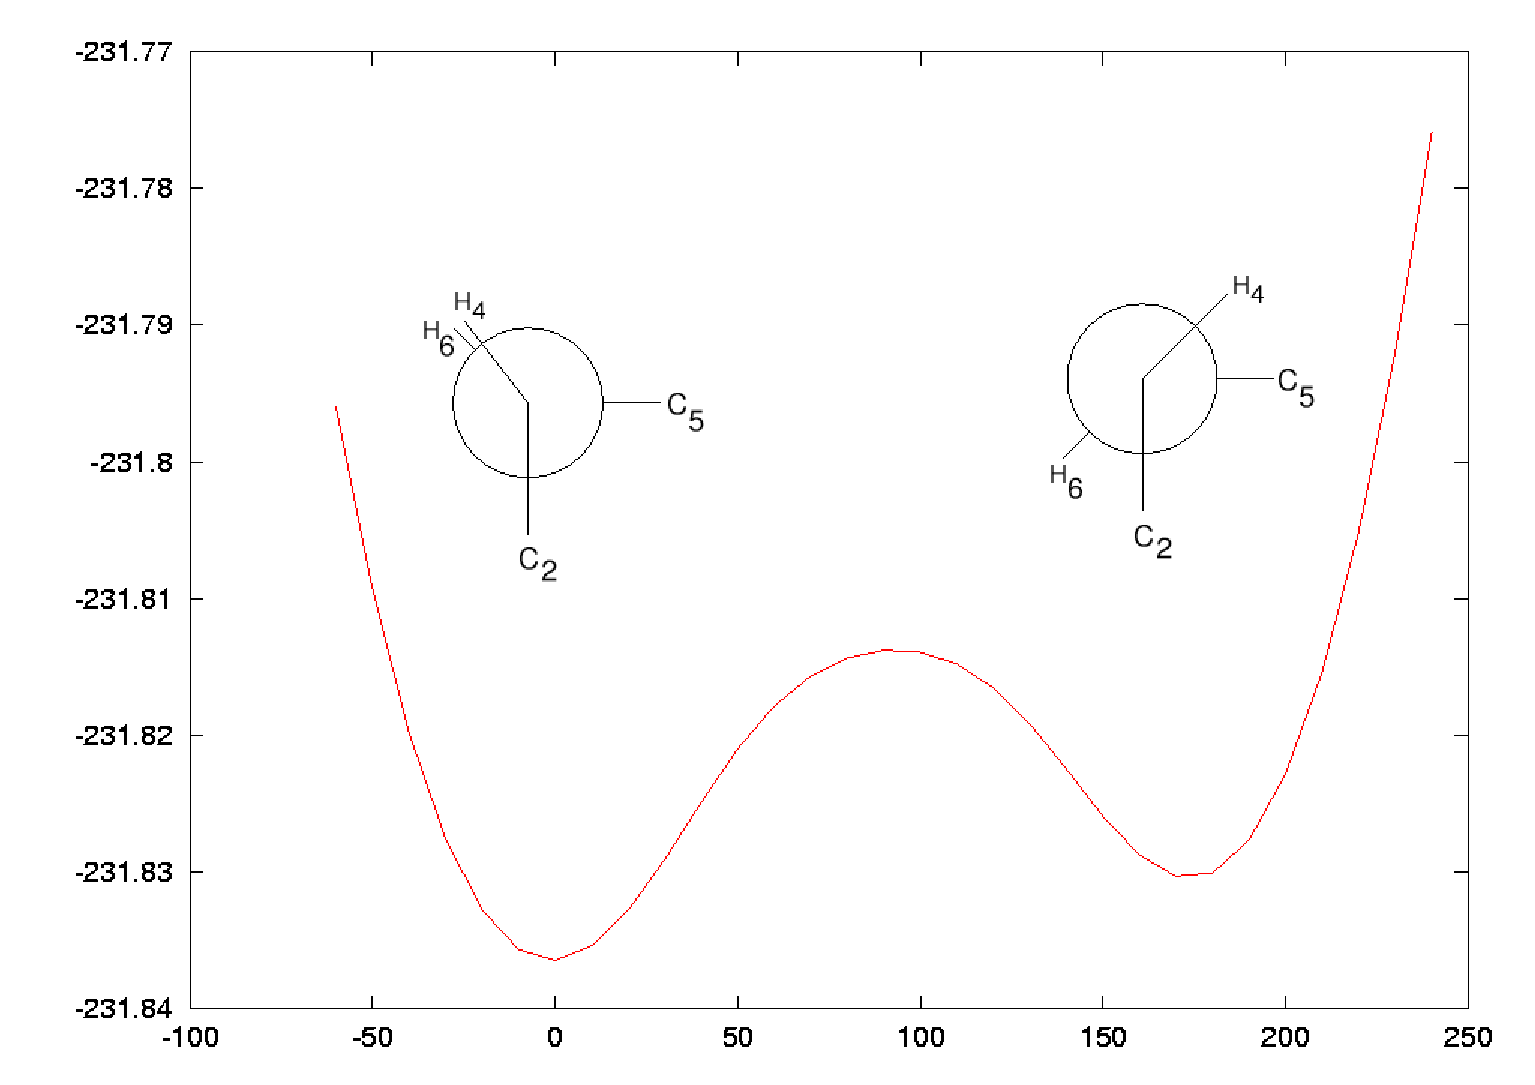
\includegraphics[width=10cm,keepaspectratio]{immagini/esatriene/c090.eps}
\end{center}
\end{figure}


Come \`e possibile notare, sono presenti due minimi, esattamente come nel
caso dell'etilene. Ciascun minimo rappresenta una possibile struttura di
equilibrio relativamente alla posizione degli idrogeni, una
approssimativamente sin-periplanare, l'altra approssimativamente
anti-periplanare. A differenza dell'etilene, tuttavia, \`e da notare che la
barriera di interconversione dalla sin alla anti \`e pi\`u bassa
(0.618 eV contro 1.45 eV per l'etilene). Questo \`e giustificabile
probabilmente in virt\`u della stabilizzazione dei due frammenti creati in
seguito alla rottura del doppio legame centrale. La formazione di due
frammenti vinilici contribuisce a ridurre l'energia della forma definita
dall'angolo diedro \mbox{H$_4$-C$_3$-C$_4$-H$_6$} a 90$^{\circ}$, in quanto tale forma
vede i frammenti privi di piramidalizzazione. Nel caso dell'etilene, si
ottenevano due orbitali $p$ completamente ortogonali che non potevano in
alcun modo interagire. Nel caso dell'esatriene e di tutti gli omologhi
superiori, ciascuno dei due orbitali \`e stabilizzato, e l'energia della
barriera risulta conseguentemente minore.

In queste condizioni, gli orbitali assumono combinazioni opportune: data la
simmetria C$_2$ della configurazione, si avranno combinazioni di simmetria
A o B sui gruppi di ciascun frammento.

Dal momento che ogni frammento pu\`o essere considerato un gruppo vinilico,
gli orbitali molecolari dello spazio attivo in questa situazione saranno 
definiti come in figura \ref{fig:esatriene_orbitali_c90_h90}
\pagebreak

\begin{figure}[htb]
\caption{\small Esatriene - spazio CAS per la configurazione con 
\mbox{H$_4$-C$_3$-C$_4$-H$_6$}=90$^{\circ}$ e
\mbox{C$_2$-C$_3$-C$_4$-C$_5$}=90$^{\circ}$ }
\label{fig:esatriene_orbitali_c90_h90}
\begin{center}
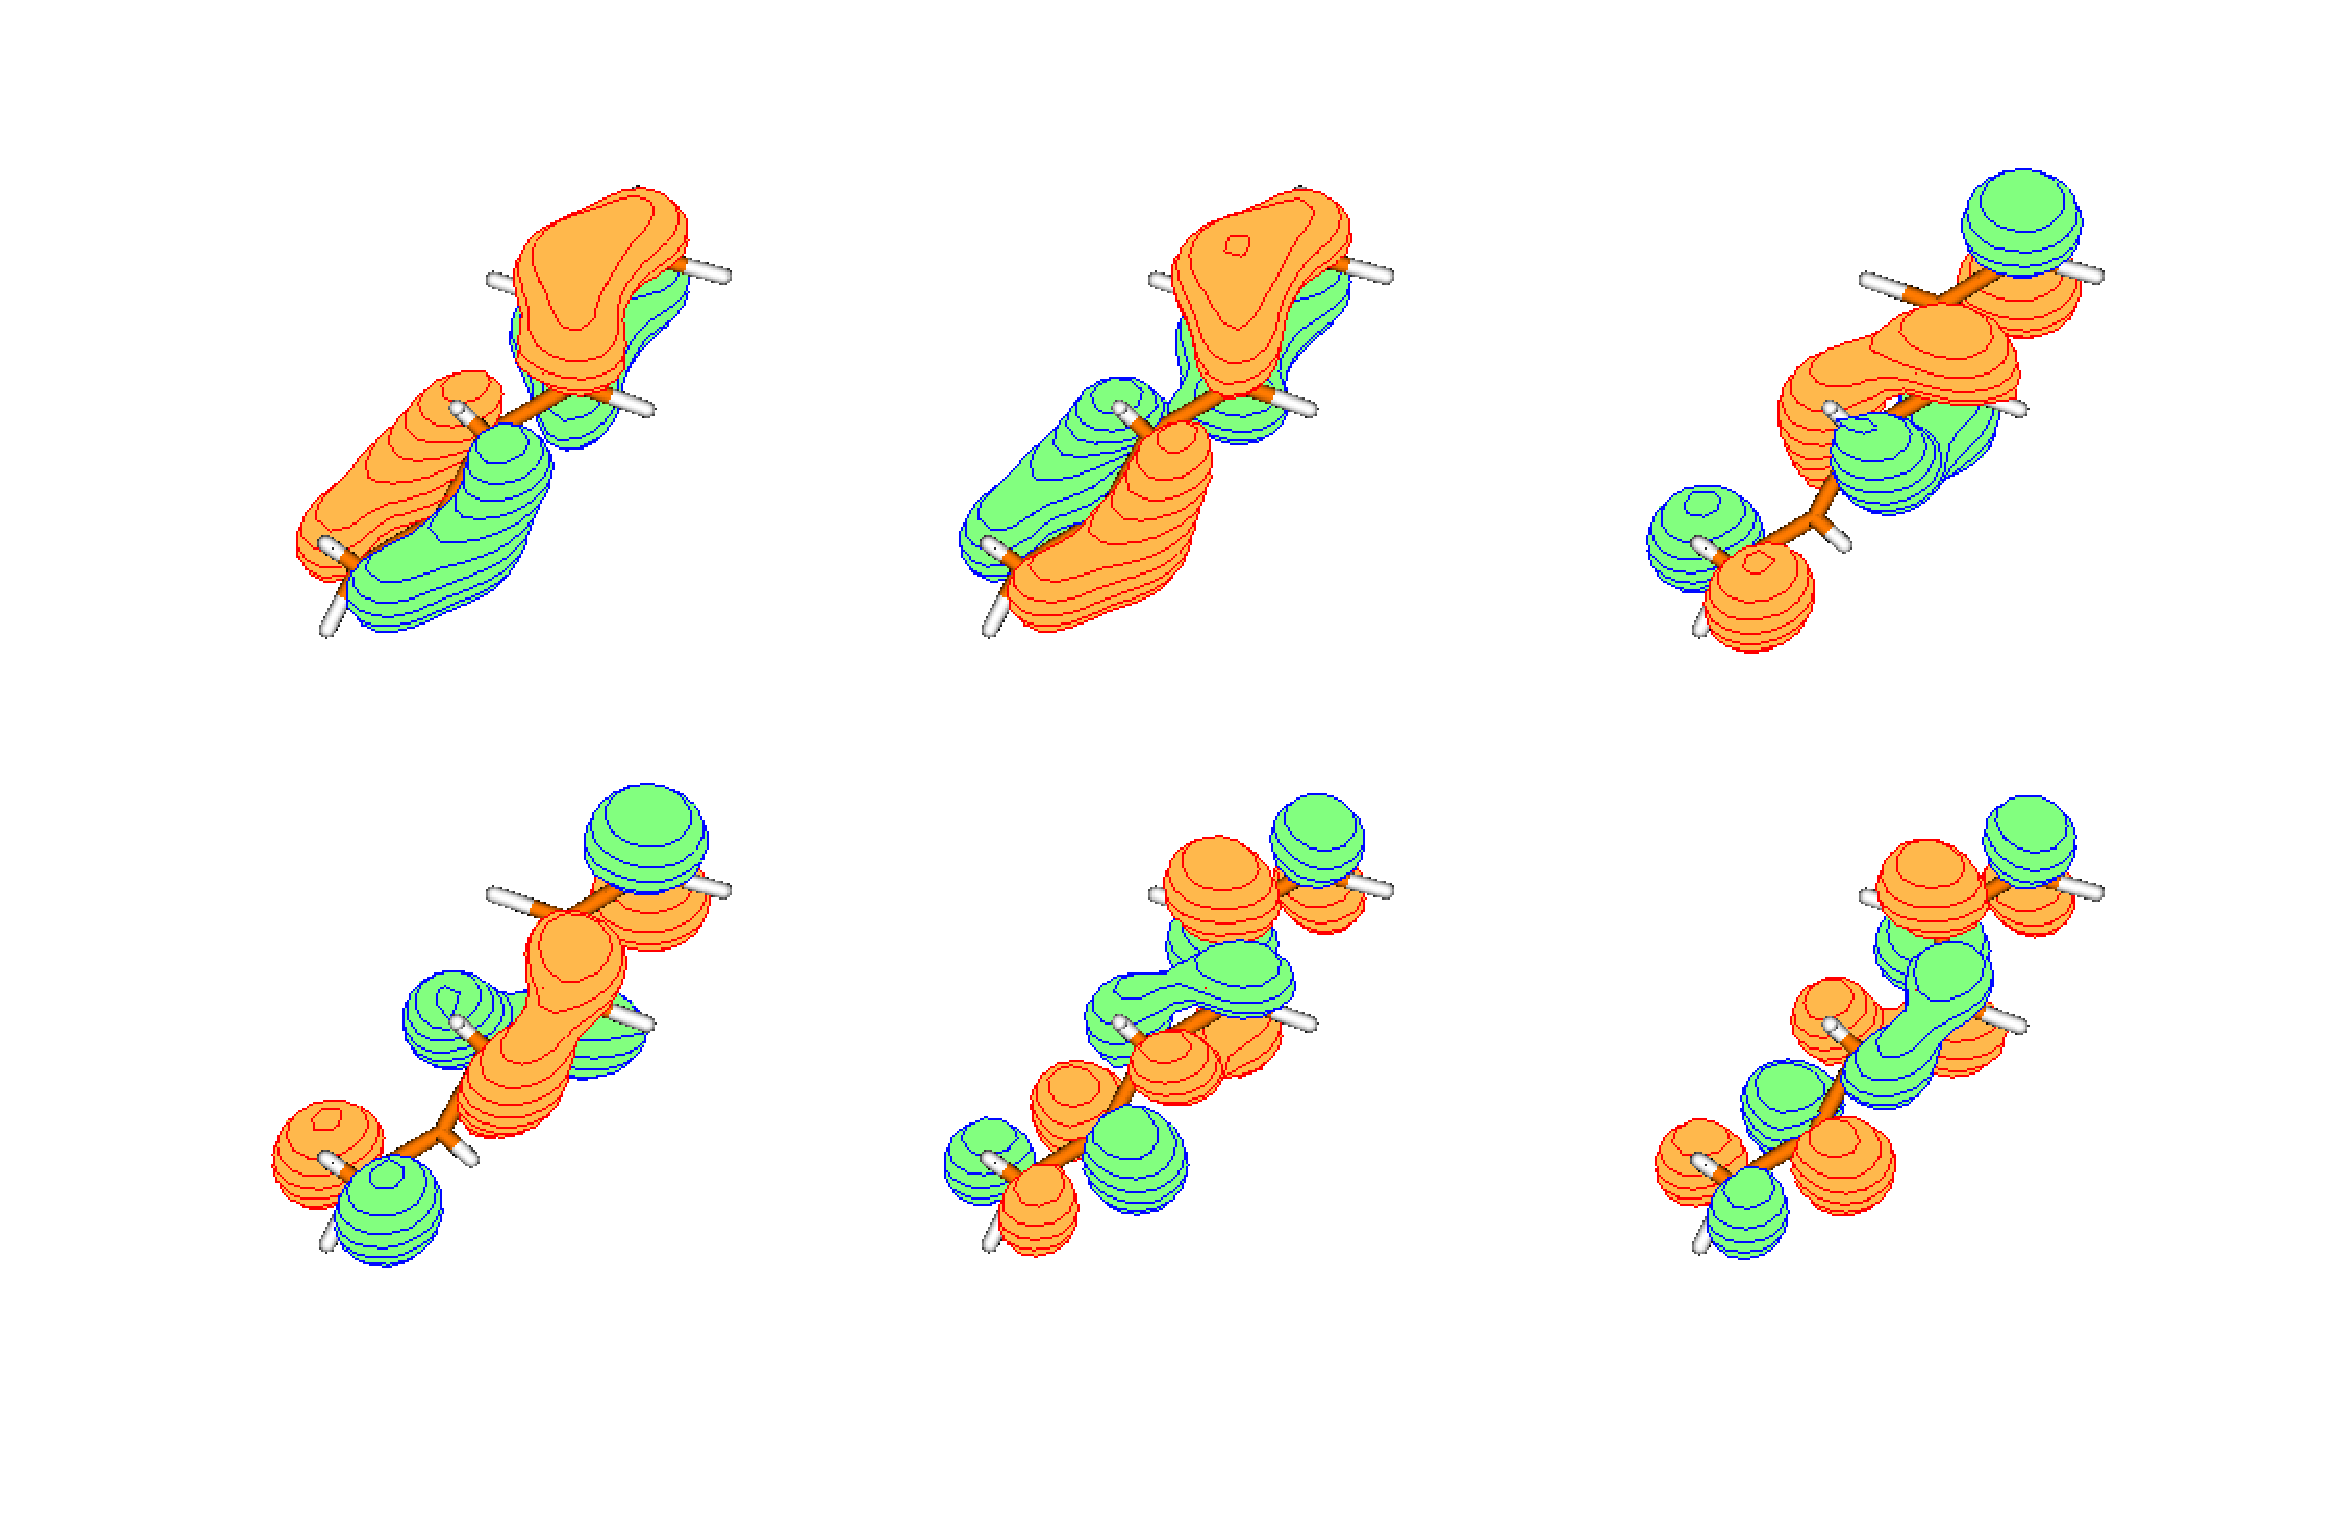
\includegraphics[width=12cm,keepaspectratio]{immagini/esatriene/orbitali_c90_h90.eps}
\end{center}
\end{figure}

Una volta ottenuto un set di orbitali per ogni posizione degli atomi di
idrogeno, si sono utilizzati come guess per ottenere le curve con angoli
diedri \mbox{C$_2$-C$_3$-C$_4$-C$_5$} inferiori e superiori di 90$^{\circ}$.

\begin{wrapfigure}{l}{8cm}
\includegraphics[angle=270,width=75mm,keepaspectratio]{immagini/esatriene/inviluppo.eps}
\caption{\small Esatriene - sezioni della superficie a vari angoli diedri C-C-C-C }
\label{fig:esatriene_inviluppo}
\end{wrapfigure}

Alcuni leggeri interventi si sono resi necessari nel caso che non si
ottenesse convergenza, tipicamente utilizzando il punto precedente o
successivo della curva. Alla fine si \`e ottenuta una superficie di
potenziale analoga a quella ottenuta per l'etilene ma, come gi\`a considerato
precedentemente, con una barriera a pi\`u bassa energia. 

\clearpage
\pagebreak

La superficie ottenuta si presta ad alcune considerazioni: \`e evidente che una
eventuale interconversione lungo questi gradi di libert\`a \`e difficilmente
realizzabile, sia perch\'e non vi \`e alcuna garanzia che questi gradi di
libert\`a siano gli unici in gioco nella interconversione, sia perch\'e questo
percorso prevede un forte spostamento di masse.

\begin{figure}[ht]
\begin{center}
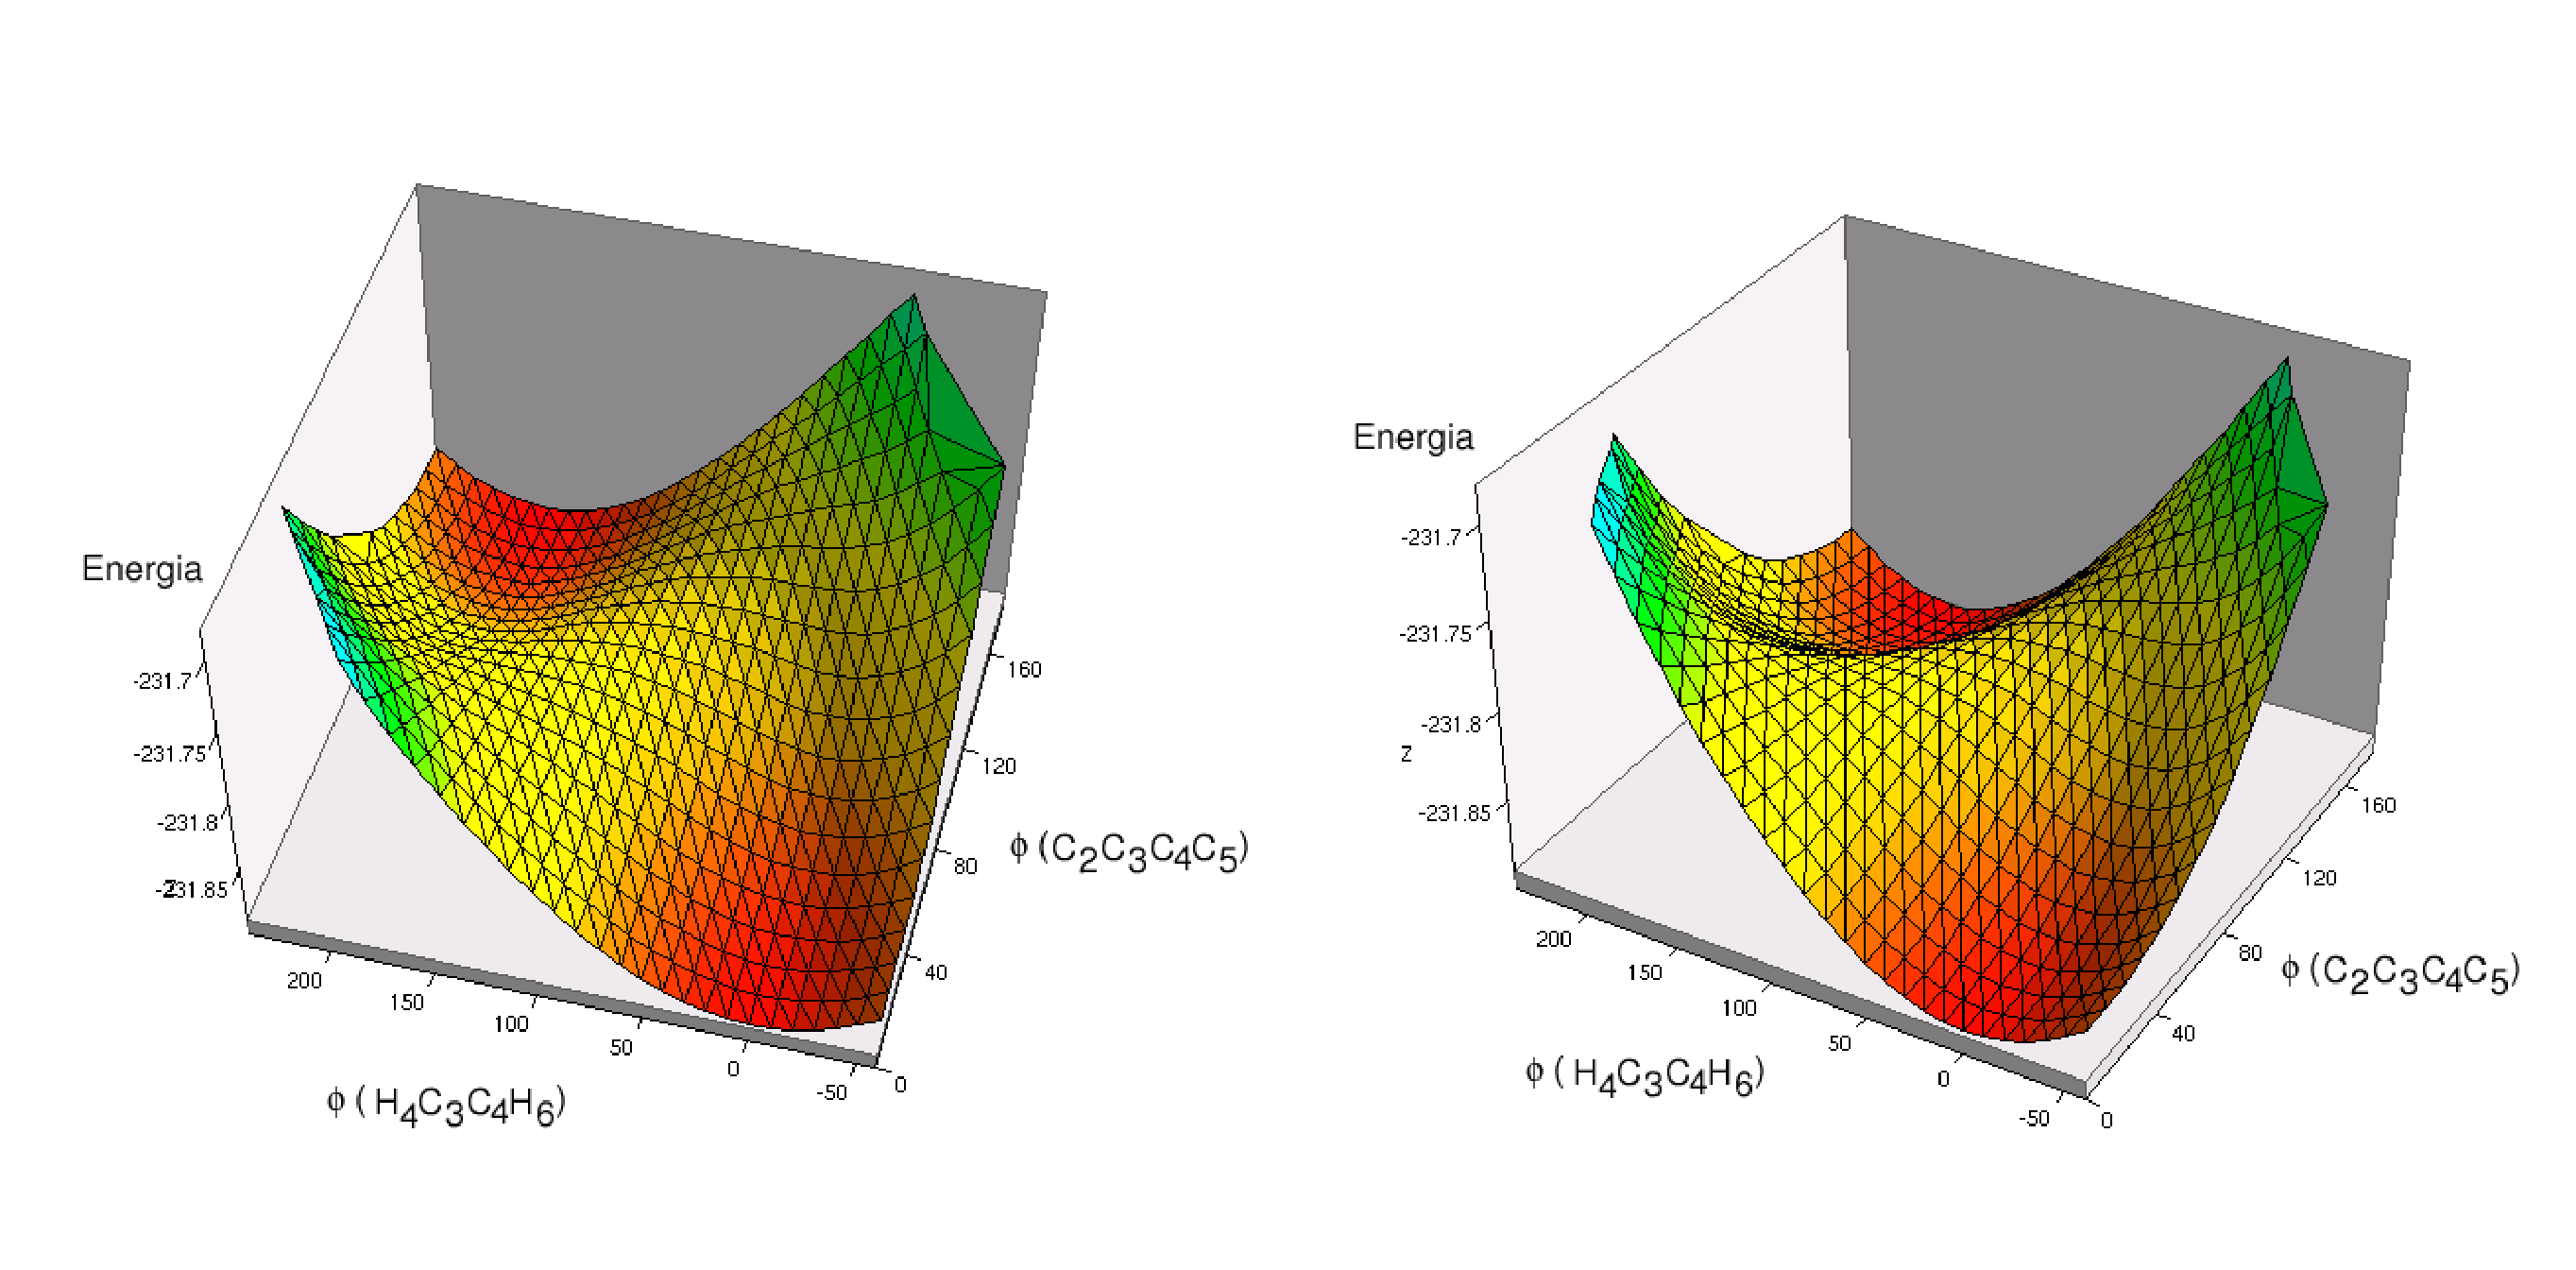
\includegraphics[angle=0,width=12cm,keepaspectratio]{immagini/esatriene/3d.eps}
\caption{\small Esatriene - superfici di potenziale}
\label{fig:esatriene_3d}
\end{center}
\end{figure}

Come conseguenza, difficilmente si tratta di una via di reale minimo energetico.
Nondimeno, una interconversione cis-trans che interessi esclusivamente lo stato
fondamentale deve necessariamente avvenire per via termica. Essendo i
polieni sistemi modello per molecole quali carotenoidi e acido retinoico,
precursori biologici di sistemi ad alta coniugazione responsabili di alcune
modalit\`a di pigmentazione e quali recettori luminosi, sar\`a centrale
nella loro interconversione il coinvolgimento di stati eccitati.
Tuttavia, \`e possibile evidenziare alcune caratteristiche interessanti:
\begin{itemize}
\item la forma sin periplanare correla, dal punto di vista strutturale, con
la forma cis del poliene. Al contrario la forma trans periplanare darebbe
origine ad un poliene i cui idrogeni centrali sono perpendicolari, e su
facce opposte, al piano molecolare, conformazione sicuramente non stabile,
come mostrato dalla ripidit\`a della curva a $\phi($C-C-C-C$) = 0^{\circ}$ e
$\phi($C-C-C-C$) = 180$.
\item analogamente, la forma trans-periplanare correla strutturalmente con
la forma trans del poliene. La forma cis-periplanare avrebbe sarebbe
analogamente non stabile, data la posizione degli idrogeni, ortogonali al
piano della molecola.
\item L'interconversione dalla forma cis ($\phi($C-C-C-C$) = 0^{\circ}$) alla forma
trans ($\phi($C-C-C-C$) = 180^{\circ}$) del poliene lungo i gradi di libert\`a definiti
impone un salto di una barriera energetica la cui altezza diminuisce via via
che l'angolo diedro $\phi($C-C-C-C$)$ aumenta. Questa barriera tende ad una
spalla che forza la risoluzione della specie verso la forma quasi
periplanare pi\`u stabile, in questo caso la trans. Analogo comportamento si
ottiene nell'interconversione dalla specie trans alla specie cis.
\end{itemize}

In virt\`u di quest'ultimo punto, il percorso di interconversione cis-trans
\`e differente dal percorso trans-cis. La molecola tende a seguire il minimo
locale della struttura che correla al meglio con lo stato di partenza, fino
a quando tale struttura non fornisce pi\`u uno stato di minimo energetico.
Quando ci\`o avviene, la struttura evolve verso lo stato di minimo energetico
modificando opportunamente la posizione degli idrogeni.

La figura \ref{fig:esatriene_mep_1} mostra i due differenti percorsi di
interconversione. Con la griglia di punti attuata per questa descrizione
(ogni 10 gradi del diedro tra i carboni)  \`e difficile localizzare dove
avvenga il rilassamento alla struttura geometricamente pi\`u stabile. Una
ulteriore difficolt\`a deriva dalla lentissima convergenza del calcolo di
ottimizzazione geometrica nelle vicinanze della spalla, punto nel quale il
gradiente \`e quasi nullo e, di conseguenza, l'eventuale riarrangiamento
verso il minimo assoluto procede molto lentamente.
La figura \ref{fig:esatriene_punti_minimo} fa riferimento alla posizione di
tali punti sul piano dei diedri.
\begin{figure}[ht]
\begin{center}
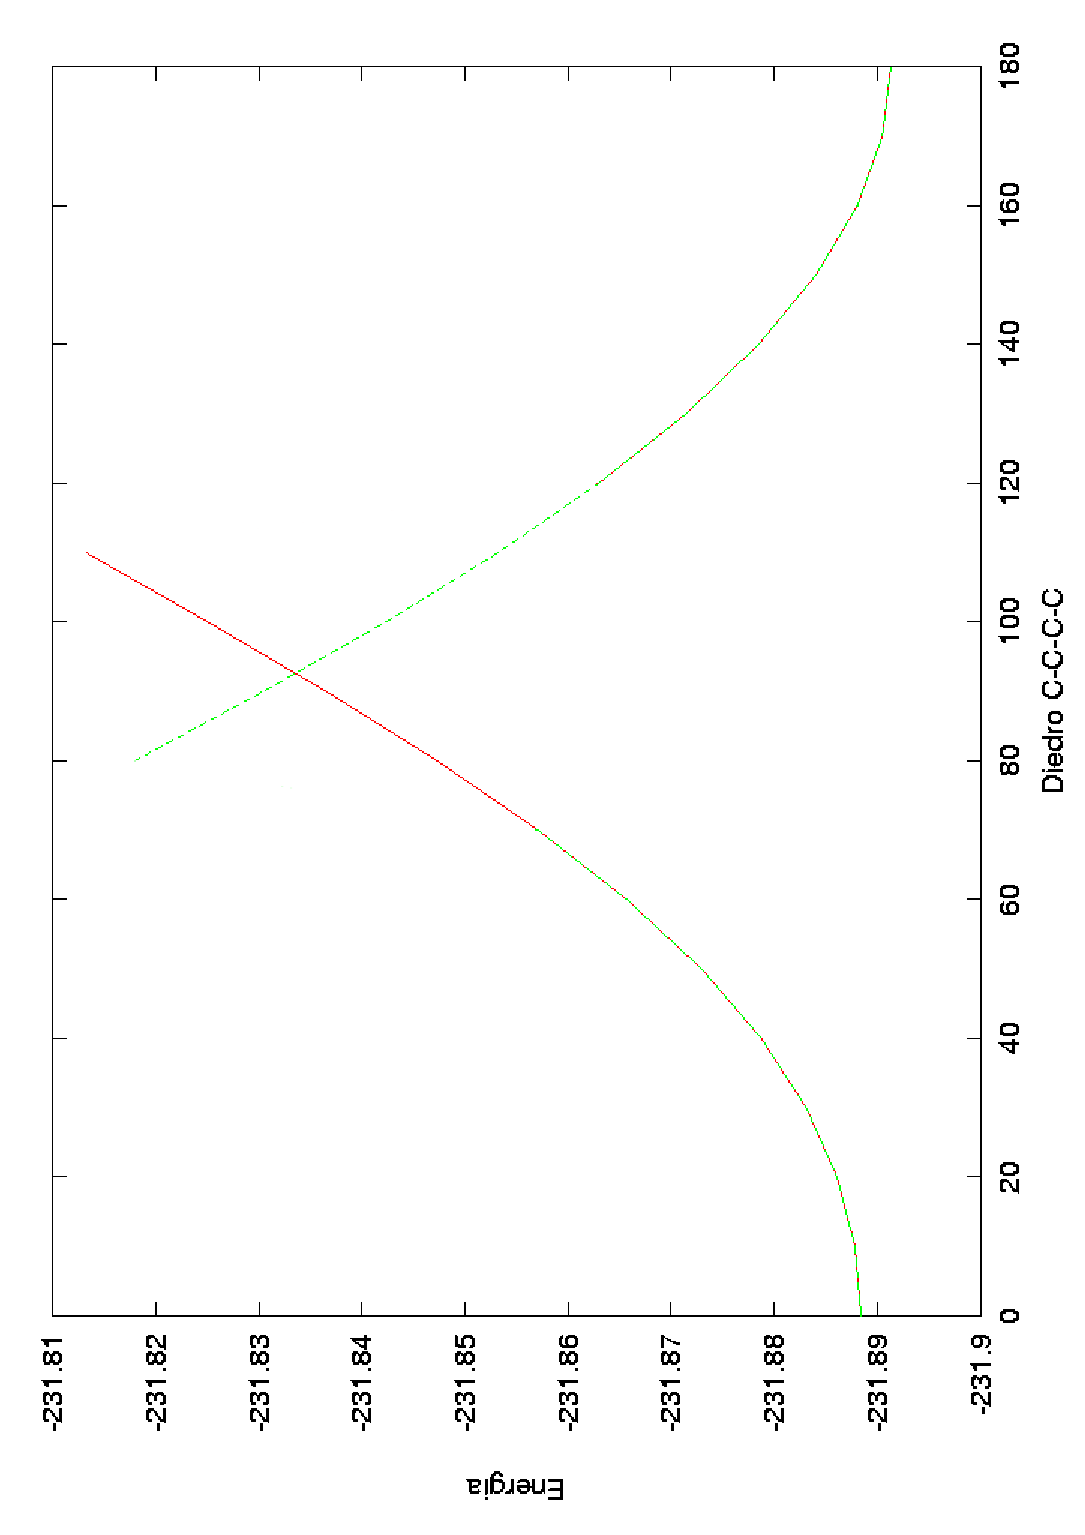
\includegraphics[angle=270,width=10cm,keepaspectratio]{immagini/esatriene/mep_1.eps}
\caption{\small Esatriene - percorso a minima energia lungo i gradi di
libert\`a definiti. Energie assolute}
\label{fig:esatriene_mep_1}
\end{center}
\end{figure}
\clearpage

\begin{figure}[ht]
\begin{center}
\includegraphics[angle=270,width=12cm,keepaspectratio]{immagini/esatriene/punti_minimo.eps}
\caption{\small Esatriene - percorso a minima energia lungo i gradi di
libert\`a definiti. Posizione sul piano definito dai diedri}
\label{fig:esatriene_punti_minimo}
\end{center}
\end{figure}

\`E quindi possibile approssimativamente definire tali punti di
interconversione in un intervallo compreso tra 70-80$^{\circ}$ per il mep
trans-cis e 110-120$^{\circ}$ per il mep cis-trans.

\subsubsection{Analisi perturbativa NEV-PT}

Successivamente allo studio approfondito a livello CASSCF, si \`e valutata
la variazione della struttura della superficie in seguito alla trattazione
perturbativa NEV-PT.

Sono state studiate le curve di potenziale rispetto al diedro H-C-C-H,
con angolo diedro C-C-C-C fissato a 0, 90 e 180$^{\circ}$. Tutte le
curve perturbative sono state traslate con opportuni valori al
fine di confrontarle dal punto di vista strutturale. Tali valori sono
di 0.710535 Hartree per le curve della trattazione strongly contracted e
0.710911 Hartree per le curve della partially contracted, valori che
rappresentano lo scarto tra le curve perturbative e la curva CASSCF nel 
punto con diedri C-C-C-C e H-C-C-H uguali a zero (ovvero la condizione di
equilibrio per l'isomero cis). 

L'analisi dell'andamento della perturbazione sulla curva a 0$^{\circ}$ ha
fornito il risultato in figura \ref{fig:esatriene_perturb_c0}.
Come si pu\`o notare, l'effetto perturbativo non introduce variazioni
nell'andamento della curva, ma si limita ad effettuare una traslazione
energetica dovuta al migliore contributo correlativo. In altri termini, il
contributo correlativo fornito dalla NEV-PT sulla funzione CASSCF \`e
uniforme per ogni punto della curva.

\begin{figure}[ht]
\begin{center}
\includegraphics[angle=270,width=12cm,keepaspectratio]{immagini/esatriene/perturb_c0.eps}
\caption{\small Esatriene - curva CASSCF (in rosso) con diedro C-C-C-C = 0$^{\circ}$, e curve perturbative
strongly (in verde) e partially (in blu), queste ultime traslate di 0.710535 e 0.710911 Hartree rispettivamente. Le
curve sono praticamente sovrapposte.}
\label{fig:esatriene_perturb_c0}
\end{center}
\end{figure}

Risultato molto simile si \`e ottenuto per la curva a 180$^{\circ}$, visibile
in figura \ref{fig:esatriene_perturb_c180}. In tale condizione \`e possibile
notare come il contributo perturbativo innalzi leggermente l'energia della
condizione pi\`u sfavorevole, ovvero quella per l'isomero trans con idrogeni
quasi ortogonali.

\begin{figure}[ht]
\begin{center}
\includegraphics[angle=270,width=12cm,keepaspectratio]{immagini/esatriene/perturb_c180.eps}
\caption{\small Esatriene - curva CASSCF (in rosso) con diedro C-C-C-C = 180$^{\circ}$, e curve perturbative
strongly (in verde) e partially (in blu), queste ultime traslate di 0.710535 e 0.710911 Hartree rispettivamente.}
\label{fig:esatriene_perturb_c180}
\end{center}
\end{figure}

Per quanto riguarda infine la curva con diedro C-C-C-C = 90$^{\circ}$,
incontriamo invece un certo cambiamento ad opera della trattazione
perturbativa: la barriera si innalza e si restringe, cos\`i come anche le due
buche di potenziale caratterizzanti i due stati coplanari per gli idrogeni. 

\begin{figure}[ht]
\begin{center}
\includegraphics[angle=270,width=12cm,keepaspectratio]{immagini/esatriene/perturb_c90.eps}
\caption{\small Esatriene - curva CASSCF (in rosso) con diedro C-C-C-C = 90$^{\circ}$, e curve perturbative
strongly (in verde) e partially (in blu), queste ultime traslate di 0.710535 e 0.710911 Hartree rispettivamente.}
\label{fig:esatriene_perturb_c90}
\end{center}
\end{figure}

\clearpage
\pagebreak

Il programma \texttt{dypc2} fornisce, nell'output, dettagli sul contributo
(come norma della correzione al primo ordine alla funzione d'onda e come energia)
sia per la correzione parzialmente contratta che
per quella fortemente contratta. Nelle figure \ref{fig:esatriene_norme_sc},
\ref{fig:esatriene_norme_pc}, \ref{fig:esatriene_energie_sc} e
\ref{fig:esatriene_energie_pc} sono mostrati rispettivamente gli andamenti,
rispetto al diedro H-C-C-H, dei valori delle norme strongly e partially e
delle correzioni alle energie strongly e partially, con diedro C-C-C-C
fissato a 90$^{\circ}$.

\`E possibile notare come il maggiore contributo alla correzione perturbativa
venga portato principalmente da $V(0)$ e $V(0')$, denotando chiaramente come 
le doppie eccitazioni siano fondamentali per la descrizione della molecola. %(Cfr. \cite{jcp-114-4-2001-1631} e \cite{jcp-112-2-2000-613})

\pagebreak
\begin{figure}[ht]
\begin{center}
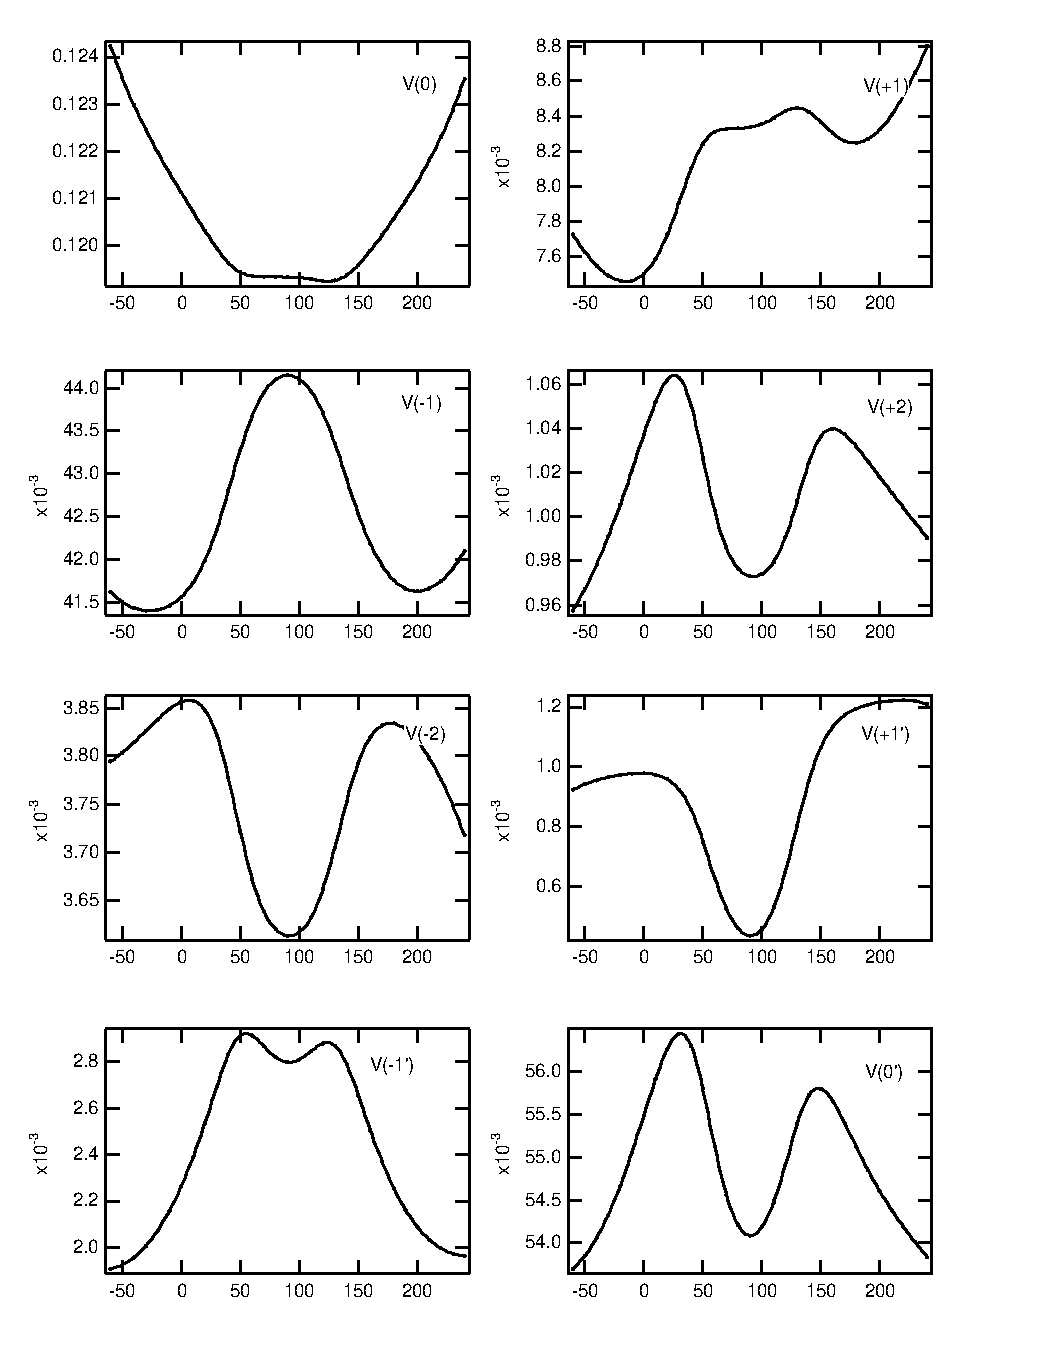
\includegraphics[angle=0,width=14cm,keepaspectratio]{immagini/esatriene/norme_sc.eps}
\caption{\small Esatriene - Norme per la correzione alla funzione d'onda.
Trattazione strongly contracted. }
\label{fig:esatriene_norme_sc}
\end{center}
\end{figure}
\pagebreak
\begin{figure}[ht]
\begin{center}
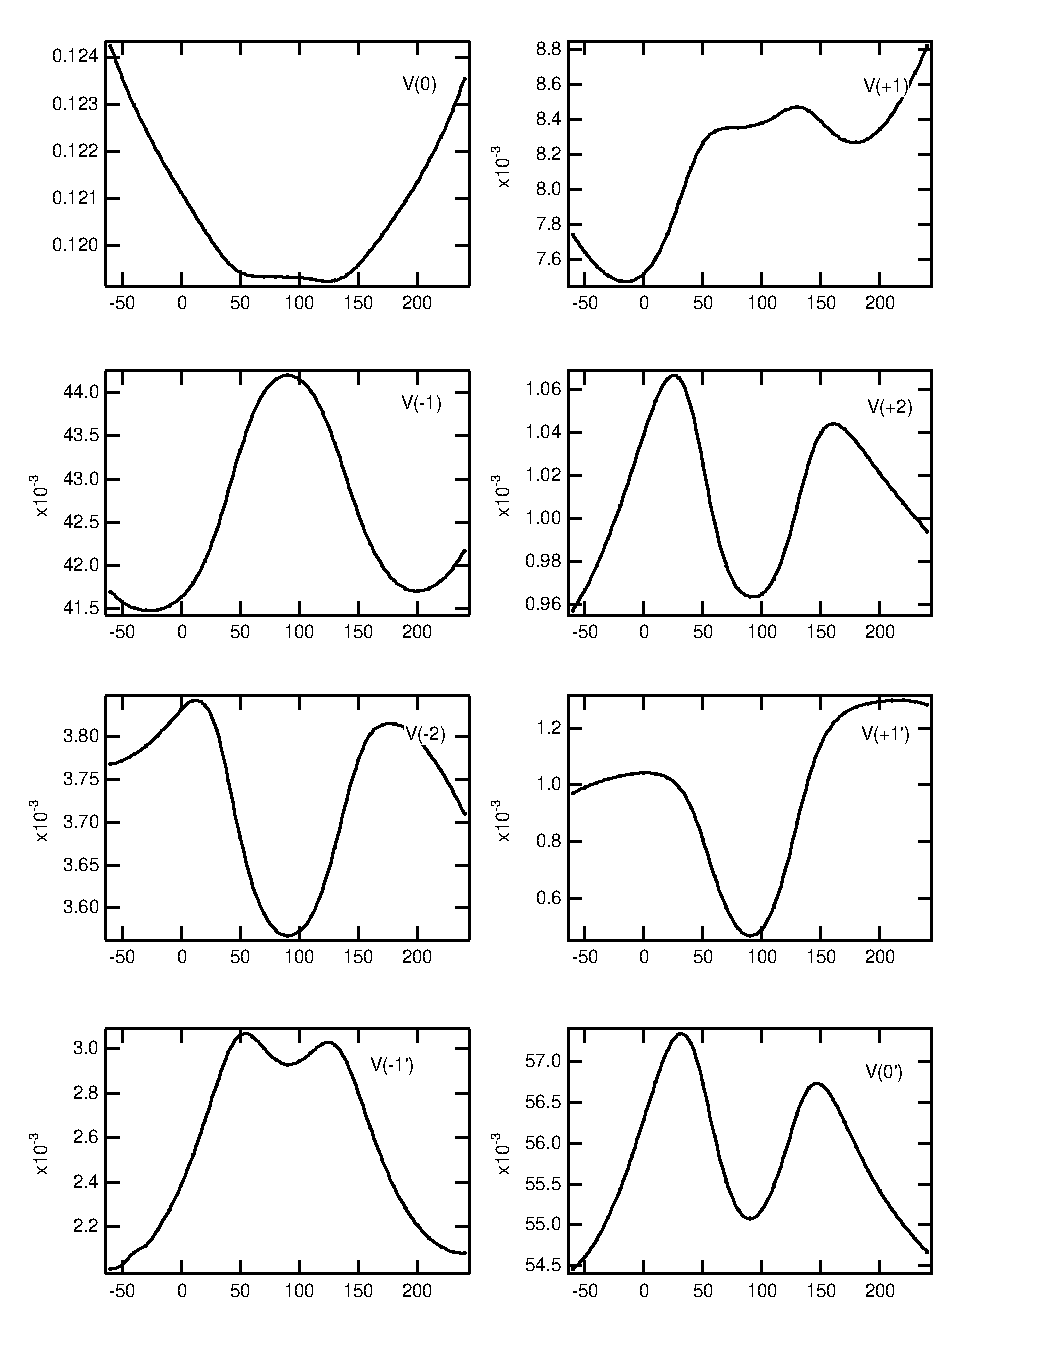
\includegraphics[angle=0,width=14cm,keepaspectratio]{immagini/esatriene/norme_pc.eps}
\caption{\small Esatriene - Norme per la correzione alla funzione d'onda.
Trattazione partially contracted. }
\label{fig:esatriene_norme_pc} 
\end{center}
\end{figure}
\pagebreak
\begin{figure}[ht]
\begin{center}
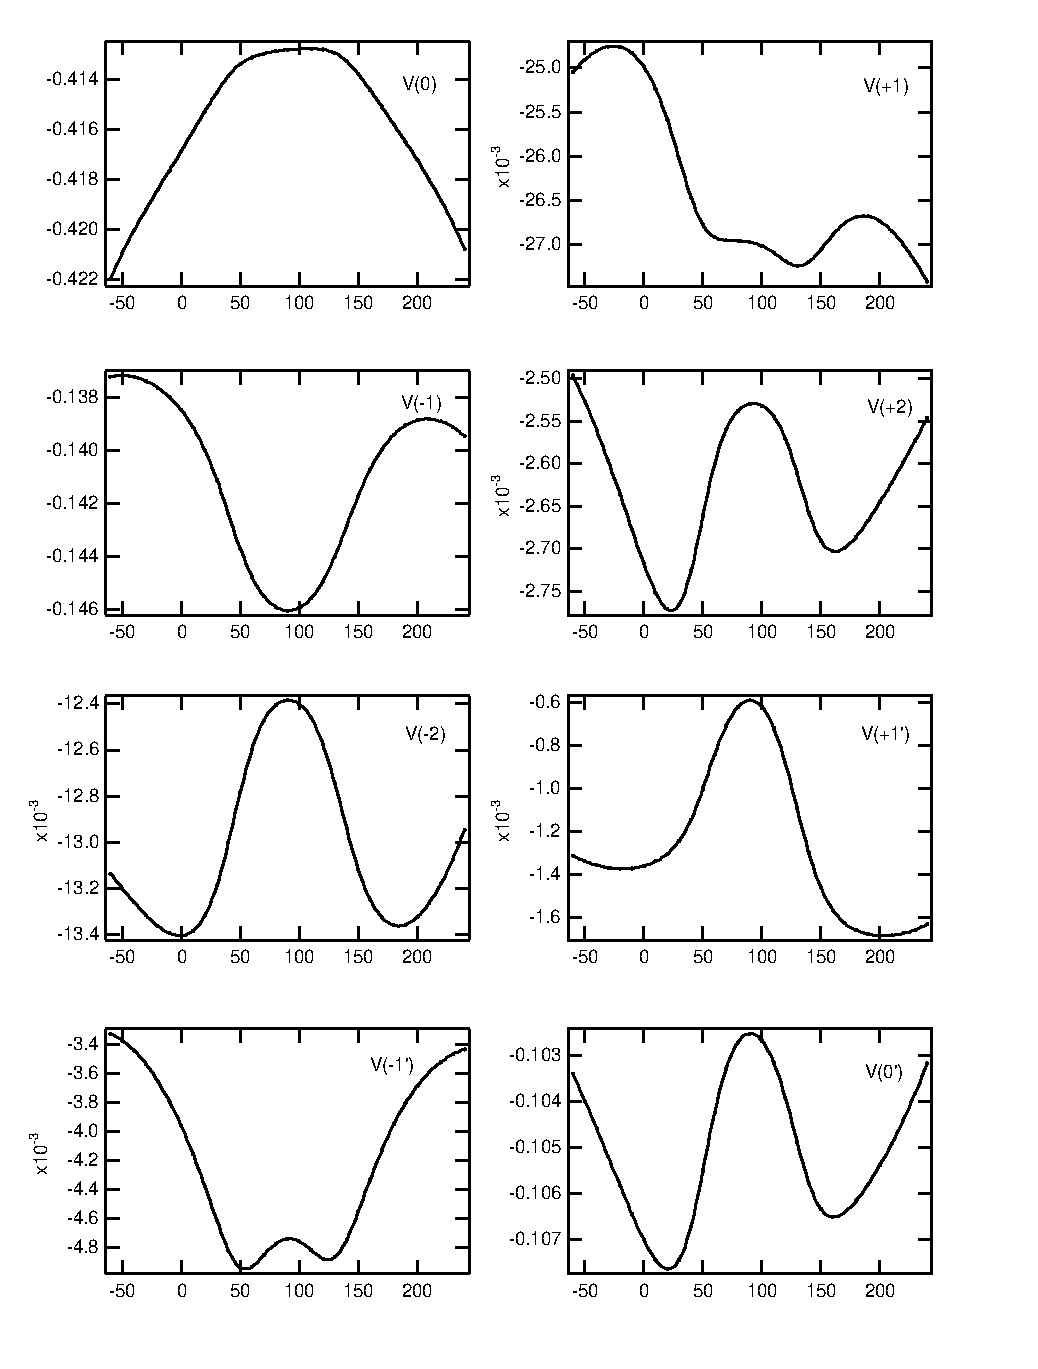
\includegraphics[angle=0,width=14cm,keepaspectratio]{immagini/esatriene/energie_sc.eps}
\caption{\small Esatriene - Contributi all'energia per l'applicazione
strongly contracted. Valori in Hartree. }
\label{fig:esatriene_energie_sc}
\end{center}
\end{figure}
\pagebreak
\begin{figure}[ht]
\begin{center}
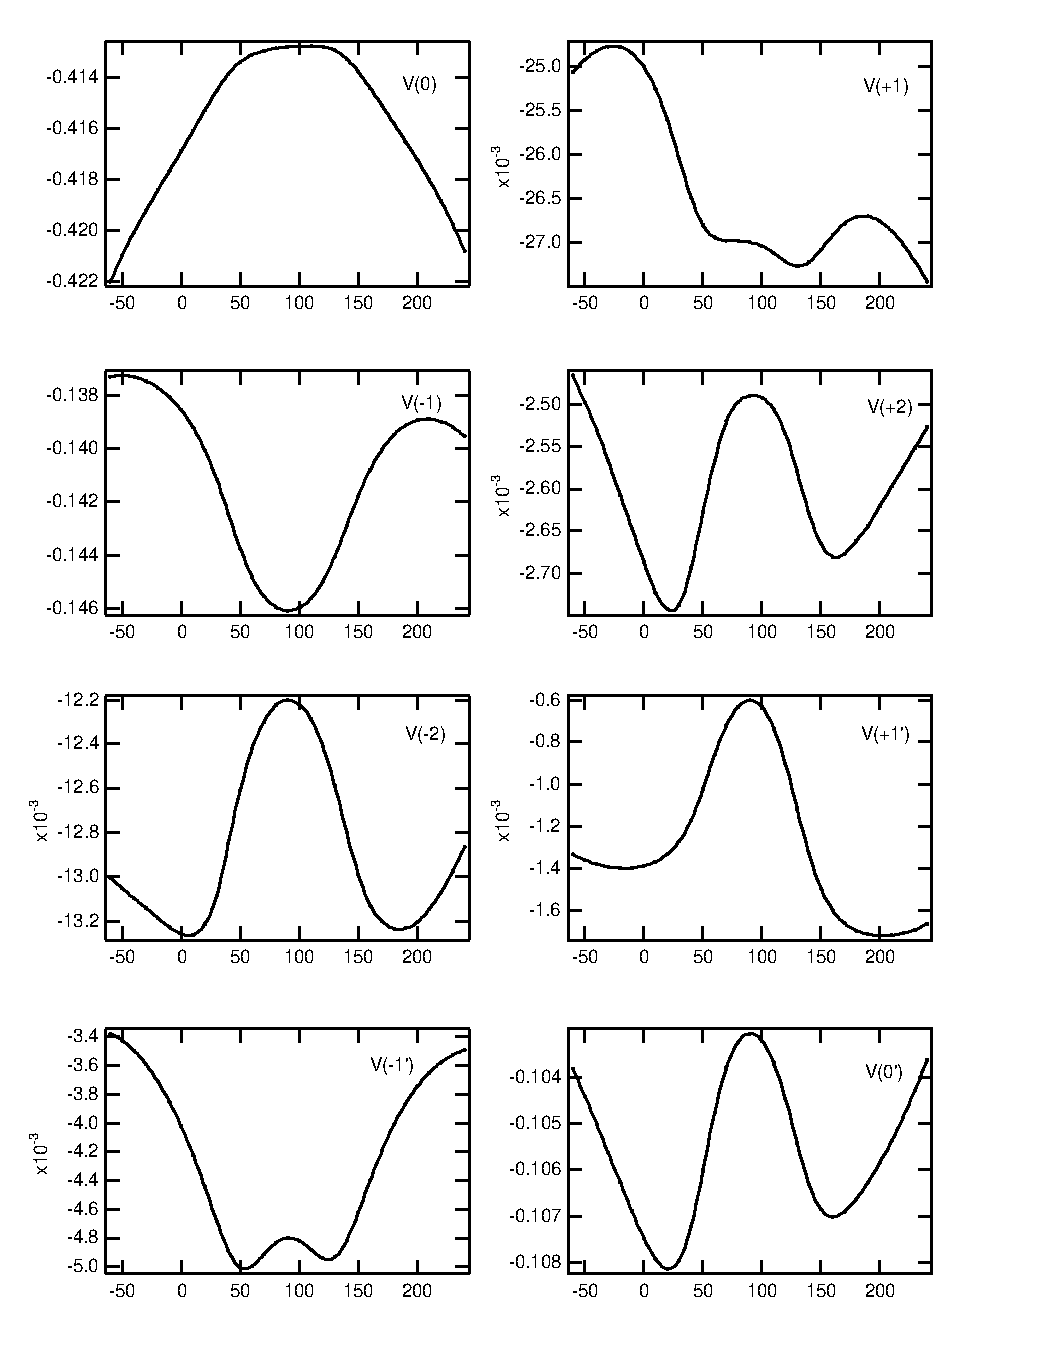
\includegraphics[angle=0,width=14cm,keepaspectratio]{immagini/esatriene/energie_pc.eps}
\caption{\small Esatriene - Contributi all'energia per l'applicazione
partially contracted. Valori in Hartree. }
\label{fig:esatriene_energie_pc}
\end{center}
\end{figure}
\pagebreak

\clearpage

\subsubsection{Energie di eccitazione verticale}

Sempre sulla molecola di esatriene si sono effettuati calcoli di valutazione
dell'energia di eccitazione verticale sia sull'isomero cis che sull'isomero
trans.

L'isomero cis, con simmetria $C_{2v}$, \`e stato ottimizzato con base 6-31G*
a livello CAS. Lo spazio attivo \`e costituito dai 6 elettroni
negli orbitali di natura $\pi$, orbitali appartenenti alle rappresentazioni
B$_1$ e A$_2$. La trattazione ha richiesto 92 configurazioni.
Al termine della procedura CASSCF, i numeri di occupazione per lo stato
fondamentale erano i seguenti
\begin{verbatim}
 Simmetria B1

   1.937856768   1.862253783   0.085298882

 Simmetria A2

   1.913147630   0.144502101   0.056940836
\end{verbatim}

Alla medesima geometria \`e stato condotto successivamente il calcolo per lo
stato eccitato 2A$_1$. I numeri di occupazione risultano essere
\begin{verbatim}
 Simmetria B1

   1.836468224   1.016224575   0.339483529

 Simmetria A2

   1.661825866   1.015253102   0.130744704
\end{verbatim}

\`E evidente la diversa distribuzione elettronica in questo stato eccitato.
A questo livello, l'energia di transizione risulta essere di 5.71 eV. Il
valore sperimentale \`e incerto, sebbene esistano alcuni riferimenti
(Cfr. \cite{jcp-114-4-2001-1631}) che forniscono un range da 4.57 a 5.04 eV.
Applicando la trattazione perturbativa, il risultato non cambia
notevolmente: l'approccio strongly contracted fornisce 5.69 eV, mentre il
partially contracted 5.67 eV. 

La medesima procedura \`e stata svolta per l'isomero trans, di simmetria
C$_{2h}$, relativamente allo stato eccitato 2$A_g$. Riferimenti esistenti
forniscono valori approssimativi, che spaziano in un range da
4.26 fino anche a 6.45 eV (vedere \cite{pccp-3-2001-2567}, \cite{jcp-112-2-2000-613},
\cite{jcp-92-1990-4622}). Il calcolo \`e stato condotto su base 6-31G* con
spazio CAS 6/6, ed il risultato ottenuto \`e 5.68 eV. A livello perturbativo,
il risultato resta sostanzialmente invariato: 5.68 eV su strongly contracted e
5.67 eV su partially.

Al fine di valutare meglio questa transizione, si \`e fatto uso di uno spazio
CAS espanso, ottenuto aggiungendo un orbitale virtuale per ogni simmetria.
In seguito a tale variazione, per descrivere il sistema sono ora necessarie
600 configurazioni per entrambi gli isomeri, contro le 92 dello spazio CAS
precedente.

La transizione per l'isomero cis fornisce, a livello CASSCF, 5.72 eV, e i
valori ricavati dalla trattazione perturbativa sono 5.74 e 5.72 eV, 
rispettivamente per strongly e partially.
L'isomero trans invece fornisce 5.69 eV, 5.73 e 5.70 rispettivamente per
CASSCF, strongly e partially.
